\documentclass[adraft, copyright, creativecommons]{eptcs} % TODO: Change to submission at the end
\providecommand{\event}{TERMGRAPH 2022} % Name of the event you are submitting to
% \usepackage{breakurl}             % Not needed if you use pdflatex only.
\usepackage{underscore}           % Only needed if you use pdflatex.

% My packages
\usepackage{orcidlink} % Orcid links
\newcommand\Mark[1]{\textsuperscript#1}

% Footnotes inside tables
\usepackage{footnote}
\usepackage{glossaries} % Glossary
\makesavenoteenv{tabular}
\makesavenoteenv{table}
\usepackage[nameinlink]{cleveref} % Reference footnotes.
\crefname{figure}{{figure}}{figures}
\Crefname{figure}{{Figure}}{Figures}
\crefformat{footnote}{#2\footnotemark[#1]#3}
% Math
\newtheorem{definition}{Definition}
\newcommand{\definitionautorefname}{Definition}
% Acronyms
\newacronym{bpmn}{BPMN}{Business Process Modeling Notation}

\title{BPMN semantics formalization and \\ model checking using graph grammars}
\author{Tim Kräuter\Mark{*}\orcidlink{0000-0003-1795-0611}, \quad
Harald König\Mark{\textdagger}\Mark{*}\orcidlink{0000-0001-6304-6311}, \quad
Adrian Rutle\Mark{*}\orcidlink{0000-0002-4158-1644}, \quad
Yngve Lamo\Mark{*}\orcidlink{0000-0001-9196-1779}
\institute{
\Mark{*}Western Norway University of Applied Sciences, Bergen, Norway
}
\institute{
\Mark{\textdagger}University of Applied Sciences, FHDW, Hannover, Germany}
\email{tkra@hvl.no, harald.koenig@fhdw.de, aru@hvl.no, yla@hvl.no}
}
\def\titlerunning{BPMN semantics formalization and model checking using graph grammars}
\def\authorrunning{Kräuter \textit{et al.}}
\begin{document}
\maketitle

% Maximum 8 pages for the first extended abstract!
% At the end 15 pages for the proceedings.

% TODO: Semantics vs. execution semantics?

\begin{abstract}
TBD abstract
\end{abstract}

\section{Introduction}
\begin{itemize}
    \item State goals: Semantics formalization/reference implementation
    \item Easy BPMN model checking (definition of propositions using BPMN syntax!)
\end{itemize}

\section{Semantics formalization}
% \begin{itemize}
%     \item General approach: Model transformation from any BPMN file to a graph grammar. Rules are generated specifically for each file.
%     \item Go through the BPMN spec and explain the formalization similar to the structure in \cite{vangorpVisualTokenbasedFormalization2013}.
%     \item Talk about best practices that help explain why some elements have not been formalized yet (Problems with the inclusive gateway, complex gateway, etc.).
% \end{itemize}
% General approach
We have developed a novel approach with the goal to cover as many of the \gls*{bpmn} features as possible.
Our approach is summarized as a \gls*{bpmn} process model in \cref{fig:approach}.
It is based on a model transformation from \gls*{bpmn} process models to graph grammars.
Thus, our approach is \textit{generative}, i.e., it constructs a new graph grammar including rules and a start graph for each \gls*{bpmn} process model.
This is a major difference compared to other approaches such as \cite{corradiniFormalApproachAnalysis2021, vangorpVisualTokenbasedFormalization2013} where only the \gls*{bpmn} process model is transformed but the rewrite rules are fixed.
\begin{figure}[h]
    \centering
    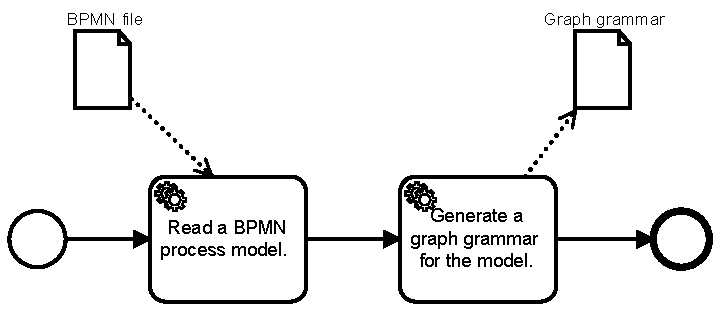
\includegraphics[width=0.5\textwidth]{images/approach-first-part.pdf}
    \caption{Semantics generation by model transformation}
    \label{fig:approach}
\end{figure}

We will now shortly introduce graph grammars before we explain the \gls*{bpmn} execution semantics formalization in detail following a similar structure as the \gls*{bpmn} specification \cite[Chapter 13]{objectmanagementgroupBusinessProcessModel2013}.

\subsection{Graph grammars}
% Shortly introduce graph grammars.
% TODO: Self plagiarism!

% Graph grammar definition
\begin{definition}[Graph grammar] \label{def:graphGrammar}
A graph grammar $GG=(S, P)$ consists of a start graph $S$ and a set of production rules $P$ \cite{ehrigFundamentalsAlgebraicGraph2006}. 
\end{definition}

The idea of a graph grammar is to begin with a start graph and then continuously apply all possible production rules.
Thus, one obtains a state space where each state is a graph, and each transition is a rule application.
Rules can be applied using different approaches, such as double-pushout (DPO) \cite{ehrigFundamentalsAlgebraicGraph2006} or single-pushout (SPO) \cite{loweAlgebraicApproachSinglepushout1993}.
Production rules for DPO are defined in \autoref{def:productionRule}.
Informally speaking, elements in $R$ but not in $L$ are added by a rule, while elements in $L$ and $R$ are preserved, and a rule deletes elements that are in $L$ but not in $R$.

% Rule definition
\begin{definition}[Production rule] \label{def:productionRule}
A production rule $P= L \overset{l}{\leftarrow} K \overset{r}{\to} R$ consists of graphs L, K, R, and graph morphisms $l: K \to L$ and $r: K \to R$ \cite{ehrigFundamentalsAlgebraicGraph2006}.
\end{definition}

% Rule application definition


% What about nested rules and nacs?

% Formalization
\subsection{Process instantiation and termination}

\subsection{Activities}
\subsection{Gateways}
% Exclusive gateway, parallel gateway, inclusive gateway, exclusive event based gateway
\subsection{Events}

% In the spec, this is below events
\subsection{Event Sub-Processes}

\section{Related work}
% \begin{itemize}
%     \item Compare the extent of the formalization in this paper with other papers formalizing BPMN semantics (Make a big table with the futures and different approaches).
%     \item Other formalizations are given in: \cite{vangorpVisualTokenbasedFormalization2013} graph transformations, \cite{wongProcessSemanticsBPMN2008} CSP, \cite{dijkmanSemanticsAnalysisBusiness2008} Petri Nets, Maude / Rewriting logic \cite{corradiniFormalApproachAnalysis2021} and more ...
%     \item Especially talks about \cite{vangorpVisualTokenbasedFormalization2013} since it also used graph rewriting but differently: fixed set of rules vs. generated set of rules by a model transformation from bpmn + differences in the resulting tools (we read bpmn files directly).
%     \item At the end we should cover more of the semantics than any currently given approach see \cite{corradiniFormalApproachAnalysis2021} for a recent overview.
%     \item Might also be interesting to compare use to Camunda or the bpmn-js token simulator. However, these projects have different goals.
% \end{itemize}

% Van gorp
A \gls*{bpmn} formalization based on in-place graph transformation rules is given in \cite{vangorpVisualTokenbasedFormalization2013}.
The formalization covers a substantial part of the \gls*{bpmn} specification, including complex concepts such as inclusive gateway merge and compensation.
In addition, graph transformation rules are visual and thus can easily be matched to the informal description of the execution semantics in the specification \cite{objectmanagementgroupBusinessProcessModel2013}.
The fixed set of graph transformation rules was implemented in a prototype using GrGen.NET \cite{vangorpVisualTokenbasedFormalization2013}.
Unfortunately, the implementation is not publicly accessible anymore.

% BProve/Corradini
The tool BProVe\footnote{\url{http://pros.unicam.it/bprove/}} is based on formal \gls*{bpmn} semantics given in rewriting logic and implemented in the Maude system.
Using these semantics, BProVe enables the verification of temporal properties for process models.
Furthermore, the tool is easily accessible online and includes multiple predefined properties, such as checking for dead activities and process completion \cite{corradiniFormalApproachAnalysis2021}.

% First order

\Cref{tab:supportedFeatures} depicts which features of the \gls*{bpmn} execution semantics are supported by the different approaches.

% Add one more maybe from van gorp
\begin{table}[htbp]

    \caption{Features supported by BPMN semantics (features similar to \cite{vangorpVisualTokenbasedFormalization2013}).}
    \label{tab:supportedFeatures}
    \begin{tabular}{l l l l l l} % <-- Alignments: 1st column left, 2nd middle and 3rd right, with vertical lines in between
    \hline
      Feature & Van Gorp &  Corradini & Houhou & ??? & This\\
      & et al. \cite{vangorpVisualTokenbasedFormalization2013} & et al. \cite{corradiniFormalApproachAnalysis2021}& et al. \cite{houhouFirstOrderLogicSemantics2019} & ??? & paper\\
      \hline
      \textit{Instantiation and termination} & & &\\
      Start event instantiation & X & X & X & & X\\
      Exclusive event-based gateway instantiation & X & ? & & & X\\
      Parallel event-based gateway instantiation &  & ? & & & \\
      Receive task instantiation &  & ? & & & X\\
      Normal process completion & X & X & X & & X\\
      \textit{Activities} & & & & &\\
      Activity & X & X & X & & X\\
      Subprocess & X & X* & X & & X\\
      Ad-hoc subprocesses &  & ? & & &\\
      Loop activity & X & ? & & & ?\\
      Multiple instance activity &  & ? & & & \\
      \textit{Gateways} & & & & &\\
      Parallel gateway & X & X & X & & X\\
      Exclusive gateway & X & X & X & & X\\
      Inclusive gateway (split) & X & X & X & & X\\
      Inclusive gateway (merge) & X & & X & & X*\\
      Event-based gateway &  & X\footnote{Does not support receive tasks after event-based gateways.} & X & & X\\ % No timer and conditional events after event based gateway supported.
      Complex gateway & & & & &\\
      \textit{Events} &  &  &  &  & \\
      None Events & X & ? & &  & X\\
      Message events & X & ? & X &  & X\\
      Timer Events &  & ? & X &  & X*\\
      Escalation Events & & ? & &  & \\
      Error Events (catch) & X & ? & &  & \color{yellow}X\\ % Yellow means I want to support this but not implemented yet.
      Error Events (throw) & X & ? & &  & \color{yellow}X\\
      Cancel Events & X & ? & &  & \color{yellow}X\\
      Compensation Events & X & ? & &  & \color{yellow}X\\
      Conditional Events &  & ? & &  & \\
      Link Events & X & ? & &  & X\\
      Signal Events & X & ? & &  & X\\
      Multiple Events &  & & &  & \\
      Terminate Events & X & ? & X & & X\\
     Boundary Events & ? & & X\footnote{Message and timer events} &  & X\\ % To the same extent as the event support
      \textit{Event subprocess} &  &  &  &  & \\
      Message Start Event &  & & &  & X\\
      Message Start Event (non-interrupting) & & & &  & X\\
      Signal Start Event &  & & &  & X\\
      Signal Start Event (non-interrupting) &  & & &  & X\\
      Other Start Events &  & & &  & \\ % Conditional and Escalation.
    \end{tabular}

\end{table}

% Summarize the findings and explain them in more detail
% Our semantics should be the most complete to date
% Our semantics is also quite understandable, i hope.

\section{Model checking BPMN}
Model checking a \gls*{bpmn} process model is straightforward after a graph grammar describing its execution semantics has been generated.
\Cref{fig:modelChecking} depicts the inputs and outputs of model checking.

\begin{figure}[h]
    \centering
    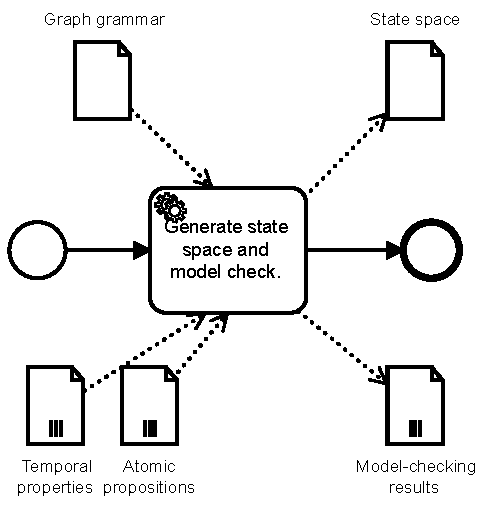
\includegraphics[width=0.4\textwidth]{images/approach-second-part.pdf}
    \caption{Model checking using graph grammars}
    \label{fig:modelChecking}
\end{figure}

Besides a graph grammar, a set of temporal properties to be checked and the atomic propositions used in the properties are supplied.
Atomic propositions must be formalized as graphs that can be matched to each state in the state space.
An atomic proposition holds in a state if and only if the graph associated with the atomic proposition is a subgraph of the graph associated with the state. % Cite groove/rensink here.
This enables model checking of temporal properties using the defined atomic propositions.

% Defining atomic propositions in BPMN is a novelty.
Since we want to hide as much complexity as possible from a user who is model checking his \gls*{bpmn} process model, we let them define atomic propositions using the familiar \gls*{bpmn} syntax.
\gls*{bpmn} is usually explained and formalized using tokens, which flow through the process model.
Thus, to define an atomic proposition, we let the user attach tokens to his \gls*{bpmn} process model, which we can automatically convert to a graph condition.

For example, the token distribution shown in \cref{fig:atomicProposition} defines two running process instances with a token in task A/B.
Differently colored tokens belong to different process instances.
This visualization was significantly inspired by the excellent bpmn-js-token-simulation\footnote{\url{https://github.com/bpmn-io/bpmn-js-token-simulation}}.
% TODO: Implement this

% TODO: Change the picture to svg once implemented etc.
\begin{figure}[h]
    \centering
    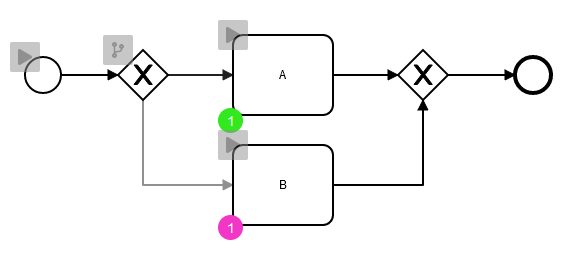
\includegraphics[width=0.6\textwidth]{images/atomicProposition.png}
    \caption{Token distribution defining an atomic proposition}
    \label{fig:atomicProposition}
\end{figure}

% \begin{itemize}
%     \item Graph grammar generates state space.
%     \item Graph conditions can be used to add atomic propositions to the state space.
%     \item We generate graph-conditions based on BPMN syntax (a big part of the novelty since this increases usability.)
%     \item Temporal Logic can be used for model checking with the defined atomic propositions.
%     \item LTL properties can, for example be checked in Groove.
%     \item Might look at some soundness things as in s3 and Bprove. Can we check them easily and how?
% \end{itemize}

\section{Implementation}
% \begin{itemize}
%     \item Talk about the tool implementation.
%     \item No installation should be needed.
%     \item Model transformation from BPMN to GG, concretely
%     \item Web tool which takes a BPMN-file and generates a zip containing a graph grammar for Groove to be downloaded, i.e.
%     \item The generated GG can be used for simulation and model checking in Groove.
%     \item We could also integrate an easier way to define atomic propositions directly using BPMN syntax and not in Groove.
% \end{itemize}
\subsection{Model-transformation to Groove}
\subsection{Evaluation}
Evaluation using multiple test cases.

Add a table here which test cases cover what part of the semantics.
\section{Conclusion}

\bibliographystyle{eptcs}
\bibliography{bib} % TODO: Should be bib.
\end{document}
